$if(has-frontmatter)$
  \frontmatter
$endif$
  
  $if(title)$
  \maketitle
$endif$

\pagenumbering{roman}

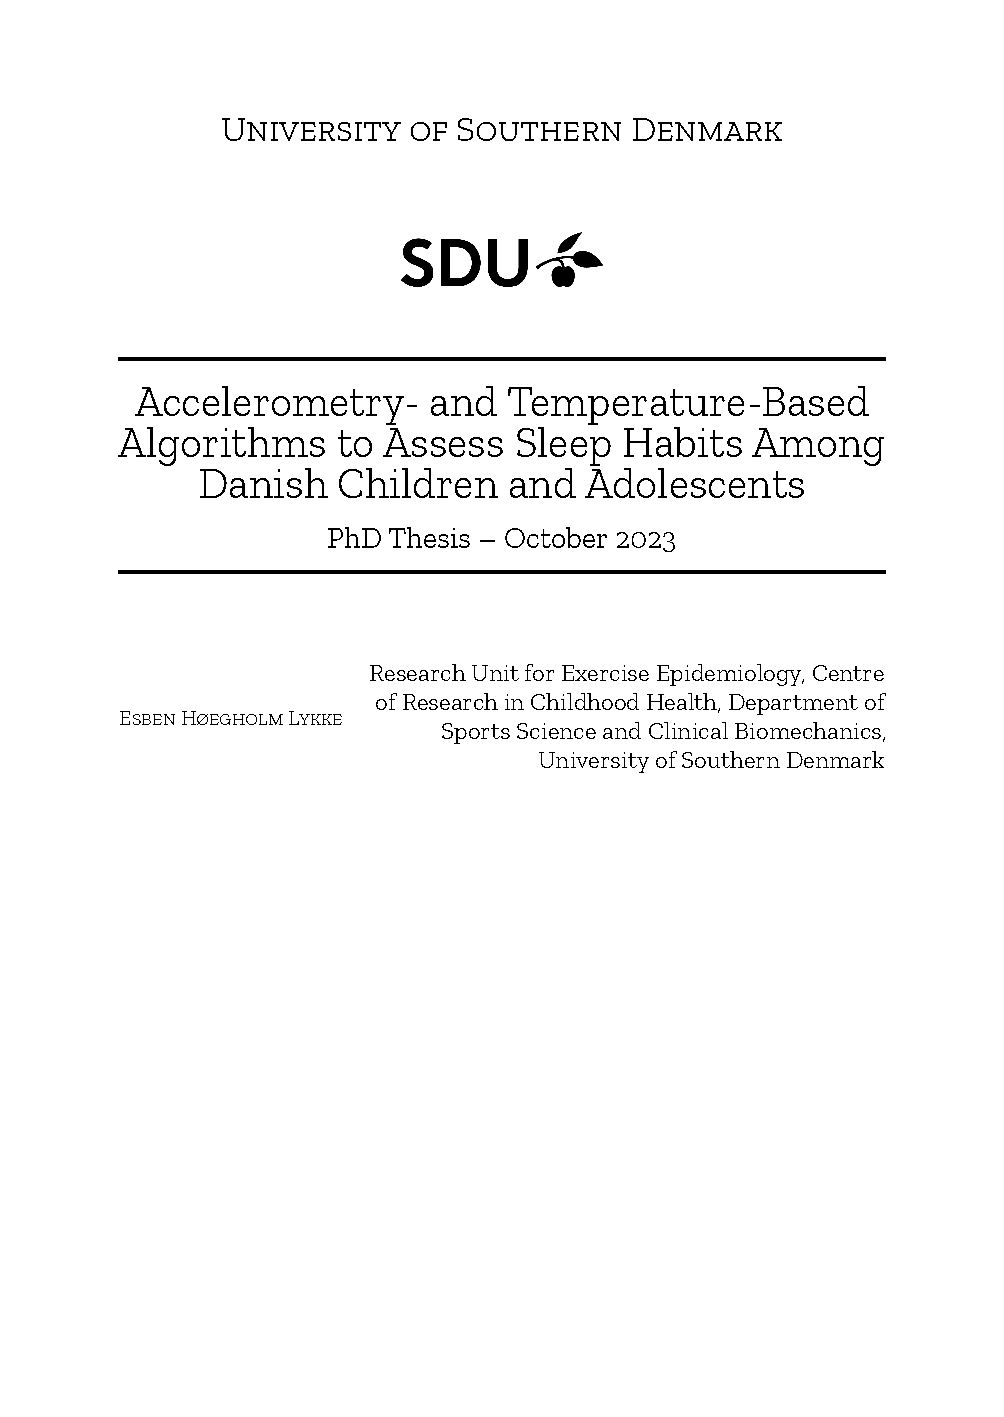
\includepdf[pages=-]{titlepage.pdf}

\newpage

\textcolor{color1}{\textsf{\textbf{\Large{Supervisor}}}}

\vspace*{\baselineskip}

Associate Professor 

Jan Christian Brønd

Research Unit for Exercise Epedimiology, Centre of Research in Childhood Health, Department of Sports Science and Clinical Biomechanics, University of Southern Denmark, Denmark

\vspace{2cm}

\textcolor{color1}{\textsf{\textbf{\Large{Assessment Committee}}}}

\vspace*{\baselineskip}

\textcolor{color1}{\textbf{Chair}}

Professor WSR 

Jasper Schiperijn

Research Unit of Active Living, Danish centre for motivation and behaviour science, Playground Research, Department of Sports Science and Clinical Biomechanics, University of Southern Denmark, Denmark

\bigskip

\textcolor{color1}{\textbf{Opponents}}

\begin{multicols}{2}

Associate Professor 

Samuel Emil Schmidt

Department of Health Science and Technology, Aalborg University, Denmark

\columnbreak

Associate Professor 

Alex Rowlands

Biomedical Research Centre, \newline University of Leicester, United Kingdom

\end{multicols}

\vspace{2cm}

\textcolor{color1}{\textsf{\textbf{\Large{Funding}}}}

\vspace*{\baselineskip}

The research presented in this thesis was generously funded by TrygFonden, under grant numbers ID 130081 and 115606, and by the European Research Council, under grant number 716657. Additional support was provided by a one-year scholarship from the Faculty of Health Sciences, University of Southern Denmark.

\newpage

%----------------------------------------------
  %   Preface
%----------------------------------------------
  
\textcolor{color1}{\textsf{\textbf{\Large{Preface}}}}

\vspace*{\baselineskip}

The present thesis delves into the objective measurements of physical behavior and sleep, a subject that has captivated me since my Master's program. This work represents a fulfilling journey marked by exploration, discovery, struggles, and both personal and professional growth.

The thesis is based on data from several different studies and is the product of collaboration with numerous internal and external co-authors. It employs machine learning and advanced statistical methods on accelerometer data to bring new insights into the field of sleep research.

This thesis comprises three distinct papers, each focusing on improving and validating methods for leveraging accelerometer data in the study of human behaviors—particularly in relation to sleep. Each paper applies innovative methods, such as machine learning techniques, to enhance the utility, reliability, and accuracy of free-living accelerometer data in large-scale studies. Two of these papers have been published in peer-reviewed journals, and the third is under preparation. These works are integral to this thesis and are included as appendices.

My research journey began during my Master's program, where I was introduced to the capabilities of accelerometer data. This early exposure culminated in the publication of my Master's thesis and solidified my desire to pursue a career in research. Embarking on my PhD, I faced a series of challenges. Initially, my limited experience with programming and machine learning posed a steep learning curve. However, persistent effort enabled me to acquire the necessary skills for this kind of work. A significant hurdle arose during the data collection phase which was intended to be used in Paper III. I attempted to collect overnight polysomnography data, along with readings from multiple accelerometers and wrist photoplethysmography, from children in their homes. Regrettably, the sensitive nature of EEG electrodes did not mix well with children, resulting in data that was largely unsuitable for model development. After gathering data from 55 children and assessing its quality, we made the difficult decision to discontinue this line of data collection. Fortunately, I could turn to the SCREENS trial for alternative data, allowing me to complete the third paper.

The PhD experience has fundamentally shaped my approach to work and life, instilling in me qualities like discipline, precision, and a keen attention to detail. This journey has been as much about professional development as it has been a personal voyage of self-discovery and growth.

As I stand on the threshold of new beginnings, I am filled with excitement about the future possibilities. This thesis reflects the lessons and experiences gathered along the way and serves as a stepping stone for further exploration in this rapidly evolving field.

Enjoy reading.

\newpage

%----------------------------------------------
  %   Acknowledgement
%----------------------------------------------
  
\textcolor{color1}{\textsf{\textbf{\Large{Acknowledgments}}}}

\vspace*{\baselineskip}

As I reflect on the transformative journey that my PhD has been, I find myself indebted to numerous individuals whose support, guidance, and inspiration have been instrumental in shaping both my professional and personal growth.
First and foremost, I extend my deepest gratitude to my Main Supervisor, Jan Christian Brønd. Your unwavering guidance and patience have not only nurtured my development as a researcher but also giving me the opportunity to lecture on interesting courses. Our collaborative dialogues, whether they took place in the office or during examinations, have been a cornerstone in my academic development.

To my co-supervisors, Anders Grøntved and Niels Christian Møller, as well as all the co-authors I've collaborated with: your expert insights and unique perspectives have immeasurably enriched my work. Even though much of our collaboration has been remote, the collegial spirit you brought forward transcended any physical distance. I deeply appreciate the camaraderie, mutual respect, and shared enthusiasm we maintained throughout our virtual interactions. While I'm grateful for how seamlessly we adapted to remote work, I do wish circumstances would have allowed for more in-person interactions and shared moments. The occasions we spent time together emphasized how much I would have loved to hang out more. I hope the future brings more opportunities for us to collaborate and connect in person.

Being part of an internationally recognized and experienced research group has been an enriching experience. It afforded me the privilege to work alongside some of the most brilliant minds in my field. This collective experience has not only broadened my understanding but also contributed significantly to our shared goal of advancing knowledge in our discipline.
My PhD journey has been about more than just academics. It's changed how I think and act in my everyday life. The careful, detailed way of doing research has affected how I make decisions and solve problems. This journey wasn't just about learning; it was also about understanding myself better. Every time I solved a tough problem, got my work published, or received good feedback, it reminded me why I'm doing this and how important it is.

At the core of this journey has been the unceasing support of my family. To my wife, who has been the bedrock of our family, your constant support and curiosity about my work have been my emotional mainstay. The joy and love I've received from our four children have been ceaseless fountains of inspiration and motivation.
To end, I want to thank everyone who helped me during my PhD—my supervisors, coworkers, friends, and family. Your support and belief in me kept me going. I hope the work in this thesis shows how much your help meant to me.

I am incredibly grateful for all the support and wisdom I have been fortunate to receive, and it is my earnest hope that this thesis stands as a tribute to each of you. Thank you.

\newpage

\textcolor{color1}{\textsf{\textbf{\Large{Included Papers}}}}

\vspace{2cm}

\begin{center}

Paper I

\textsf{Manual Annotation of Time in Bed Using Free-Living Recordings of Accelerometry Data}

published in \href{https://doi.org/10.3390/s21248442}{Sensors}

\vspace{2cm}
Paper II

\textsf{Generalizability and Performance of Methods to Detect Non–Wear with Free–Living Accelerometer Recordings}

published in \href{https://doi.org/10.1038/s41598-023-29666-x}{Scientific Reports}

\vspace{2cm}
Paper III 

\textsf{Improving Sleep Quality Estimation: A Comparative Study of Machine Learning and Deep Learning Techniques Utilizing Free–Living Accelerometer Data from Thigh-Worn Devices and EEG-Based Sleep Tracking}

In preparation for \href{https://academic.oup.com/sleep}{SLEEP}

\end{center}
